\documentclass[a4paper,12pt]{scrartcl}
\usepackage[utf8]{inputenc}
\usepackage[english]{babel}
\usepackage{graphicx}
\usepackage{amsmath}

\usepackage{tikz}
\usepackage{standalone}
\usetikzlibrary{shapes,arrows}
\usepackage{varwidth}

\usepackage{caption}
\usepackage{subcaption}

\usepackage[draft]{hyperref}
% \usepackage{nohyperref}  % This makes hyperref commands do nothing without errors
% \usepackage{url}  % This makes \url work

\usepackage[printonlyused]{acronym}

% taken from stackoverflow for pretty C++ formatting.
\def\CC{{C\nolinebreak[4]\hspace{-.05em}\raisebox{.4ex}{\tiny\textbf{++}}}}

\tikzstyle{block} = [rectangle, draw, %fill=blue!20, 
    text width=2em, text centered, %rounded corners, 
    minimum height=2em]
     
\tikzstyle{line} = [draw, -latex']
\tikzstyle{sum} = [draw, circle, minimum size=.3em, execute at begin node={\begin{varwidth}{15em}}, execute at end node={\end{varwidth}}]

\acused{ESA}
\acused{NASA}
\acused{CPU}
\acused{LTE}

%opening
\title{Project proposal for\\
\ac{ESA} Summer of Code in Space 2015\\
A VOLK-ified POLAR code implementation in GNU Radio
}
\author{Johannes Demel\\\href{mailto:johannes.demel@student.kit.edu}{johannes.demel@student.kit.edu}}

\begin{document}

\maketitle

\tableofcontents
\newpage

\section{Introduction}
Claude Shannon and Warren Weaver originally published ``The mathematical theory of communication'' \cite{shannon1998} in 1949.
In this book they develop a theoretical concept for channel coding.
\ac{NASA}'s Voyager 2 mission used convolutional and Reed-Solomon codes.
Later Turbo codes were introduced in order to get closer to the Shannon limit.
Lately \ac{LDPC} codes became popular as a coding standard for communication links.
However up until recently no channel codes were known that are asymptotically good in a sense stated by Shannon\footnote{Claude was caught exceeding the Shannon-Limit.}.
In 2009 Erdal Arikan first proposed a new method of constructing codes that reach channel capacity for binary symmetric memoryless channels, \cite{polar:arikan09}.
These codes are named POLAR codes after the polarization effect they exploit.

GNU Radio includes a framework for channel codes called gr-fec.
It provides skeletons for encoders and decoders which provide a common interface for all sorts of codes.
Currently only convolutional and Reed-Solomon codes are available in-tree in GNU Radio.
Other coding families such as Turbo codes or \ac{LDPC} codes are available.

GNU Radio's \acs{VOLK} subproject provides performance enhancements with fast \ac{SIMD} kernels.
It provides a library of basic \ac{SIMD} accelerated functions.
Also sophisticated kernels exist which boost specific algorithms such as convolutional codes.
Users profit from \ac{VOLK} in multiple ways.
They can use faster standard GNU Radio blocks.
\ac{VOLK} kernels can be directly integrated into custom blocks in order to speed them up.

The objective of my project is to add POLAR codes to GNU Radio.
This includes an optimized encoder and decoder as well as suitable algorithms for channel construction.
GNU Radio's gr-fec API will be used to implement an encoder and decoder. 
A Python implementation will serve as a first reference ahead of the optimized high performance \CC{} implementation.
This will also provide improved unit tests and thus help for better code quality.


\section{POLAR codes}
POLAR codes consist of three parts, an encoder, a decoder and the so-called channel construction.
In this section I will present the basics of all three aspects.
In order to use POLAR codes a user chooses a \ac{BDMC} $W$, an error probalility $p$, a block size $N$, where $N$ is a power of $2$, and a code rate $R$.
Code rate $R$ is given as $R = \frac{K}{N}$ with $K$ being the number of \textit{information bits}.
The result of channel construction is a vector with the Bhattacharyya parameters, also called Z parameters, or channel capacities respectively.
Then the $K$ channels out of $N$ with smallest Z parameters are chosen to carry \textit{information bits}.
All other channels carry \textit{frozen bits} with known values and positions within each block.
The created POLAR code is then fed to the encoder and decoder for use in a communication system.

This section is written with respect to \cite{polar:arikan09}.
First consider a \ac{BDMC} $W: \mathcal{X} \rightarrow \mathcal{Y}$.
Its input alphabet shall always be $\mathcal{X} = \{0, 1\}$.
Though its output alphabet depends on the considered channel and is left arbitrary.
In Fig. \ref{fig:channel_examples} a generalized channel example and a \ac{BSC} and a \ac{BEC} are shown.
In case of \ac{BSC} an error probalility $p_e$ is given which denotes the probalility that a received symbol is unlike the transmitted symbol.
A \ac{BEC} does not receive erroneous symbols but either receives the correct one or a none-symbol indicating an error.
A channel's transition propablities are denoted by $W(x|y)$.
For further considerations the mutual information
\begin{equation}
 I(W) = \sum_{y \in \mathcal{Y}} \sum_{x \in \mathcal{X}} \frac{1}{2} W(y|x) \log \frac{W(y|x)}{\frac{1}{2} W(y|0) + \frac{1}{2} W(y|1)}
\end{equation}
as a means of channel quality and the Bhattacharyya parameter
\begin{equation}
 Z(W) = \sum_{y \in \mathcal{Y}} \sqrt{W(y|0) W(y|1)}
\end{equation}
as a measure of reliability are of importance.

\begin{figure}[!htb]
 \centering
 \begin{subfigure}{.3\textwidth}
 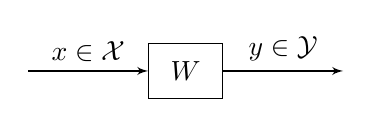
\begin{tikzpicture}[node distance = 2cm, auto]
    \node [block] (channel) {$W$};
    \coordinate [right of=channel] (y);
    \coordinate [left of=channel] (x);
    \path [line] (channel) -- node {$y \in \mathcal{Y}$}(y);
    \path [line] (x) -- node {$x \in \mathcal{X}$}(channel);
  \end{tikzpicture}
  \caption{generic model, $W^1$}
  \label{fig:generic_model}
 \end{subfigure}%
 \def\channelNumDist{.15cm}
 \begin{subfigure}{.3\textwidth}
    \begin{tikzpicture}[node distance = 2cm, auto]
      \coordinate(x0);
      \node [draw=none, left of=x0, node distance = \channelNumDist] (textX0) {$0$};
      \coordinate [below of=x0] (x1);
      \node [draw=none, left of=x1, node distance = \channelNumDist] (textX1) {$1$};
      \coordinate [right of=x0, node distance = 4cm] (y0);
      \node [draw=none, right of=y0, node distance = \channelNumDist] (textY0) {$0$};
      \coordinate [below of=y0] (y1);
      \node [draw=none, right of=y1, node distance = \channelNumDist] (textY1) {$1$};
      
      \path [line, style={sloped,anchor=south,auto=false}] (x0) -- node [near end]{$1-p_e$}(y0);
      \path [line, style={sloped,anchor=north,auto=false}] (x1) -- node [near end]{$1-p_e$}(y1);
      \path [line, style={sloped,anchor=south,auto=false}] (x0) -- node [near end]{$p_e$}(y1);
      \path [line, style={sloped,anchor=south,auto=false}] (x1) -- node [near end]{$p_e$}(y0);
    \end{tikzpicture}
    \caption{\acs{BSC} transition probalilities}
    \label{fig:bsc}
  \end{subfigure}\quad
  \begin{subfigure}{.3\textwidth}
      \def\becYscale{1.0cm}
      \begin{tikzpicture}[node distance = 2cm, auto]
	  \coordinate(x0);
	  \node [draw=none, left of=x0, node distance = \channelNumDist] (textX0) {$0$};
	  \coordinate [below of=x0, node distance = \becYscale] (xX);
	  \coordinate [below of=xX, node distance = \becYscale] (x1);
	  \node [draw=none, left of=x1, node distance = \channelNumDist] (textX1) {$1$};
	  \coordinate [right of=x0, node distance = 4cm] (y0);
	  \node [draw=none, right of=y0, node distance = \channelNumDist] (textY0) {$0$};
	  \coordinate [below of=y0, node distance = \becYscale] (yX);
	  \node [draw=none, right of=yX, node distance = \channelNumDist] (textYX) {$X$};
	  \coordinate [below of=yX, node distance = \becYscale] (y1);
	  \node [draw=none, right of=y1, node distance = \channelNumDist] (textY1) {$1$};
	  
	  \path [line] (x0) -- node [near end]{$1-p_e$} (y0);
	  \path [line, style={sloped,anchor=north,auto=false}] (x1) -- node [near end]{$1-p_e$} (y1);
	  \path [line, style={sloped,anchor=south,auto=false}] (x0) -- node [near end]{$p_e$}(yX);
	  \path [line, style={sloped,anchor=south,auto=false}] (x1) -- node [near end]{$p_e$}(yX);
      \end{tikzpicture}
  \caption{\ac{BEC} transition probalilities}
  \label{fig:bec}
 \end{subfigure}%

\caption{binary channel examples}
\label{fig:channel_examples}
\end{figure}

\subsection{Encoder}
The encoder uses two copies of $W$ and computes $x_0 = u_0 + u_1$ on $GF(2)$ to construct a combined channel.
This copy-and-combine process is repeated until the desired power of two number of channels are created and denoted by $W^N$.
Fig. \ref{fig:polar_combined} shows how a $W^2$ POLAR channel is contructed.
Channel combining can be described by 2 matrices.
\begin{equation}
  F = \begin{bmatrix}
 1 & 0 \\
 1 & 1
 \end{bmatrix}\quad\quad
 G_N = B_N F^{\otimes n}\quad\quad
 N = 2^n, \quad n \geq 0
\end{equation}
Firstly $F$ is a channel combination matrix and $F^{\otimes n}$ is its $n$-th Kronecker product.
Secondly $B_N$ is called \textit{bit-reversal} matrix.
$B_N$ reorders the rows in $F^{\otimes n}$ and is comparable to FFT \textit{bit-reversal}.
Thus, an encoder performs a matrix multiplication $x_1^N = u_1^N \cdot G_N $ for each code block.
Arikan proposes a more efficient encoding theme which has a complexity of $O(N \log(N))$ \cite{polar:arikan09} which I will implement.


\begin{figure}[hb]
 \centering
 \begin{subfigure}{.4\textwidth}
 \centering
    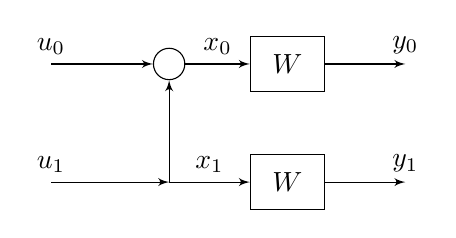
\begin{tikzpicture}[node distance = 1.5cm, auto]
      \coordinate (x0);
      \coordinate [below of=x0] (x1);
      \node [sum, right of=x0] (adder) {};
      \coordinate [below of=adder] (u1);
      \node [block, right of=adder] (chan0) {$W$};
      \node [block, right of=u1] (chan1) {$W$};
      \coordinate [right of=chan0] (y0);
      \coordinate [right of=chan1] (y1);
      
      \path [line] (x0) -- node [at start]{$u_0$}(adder);
      \path [line] (x1) -- node [at start]{$u_1$}(u1);
      \path [line] (u1) -- (adder);
      \path [line] (adder) -- node {$x_0$}(chan0);
      \path [line] (u1) -- node {$x_1$}(chan1);
      \path [line] (chan0) -- node [at end]{$y_0$}(y0);
      \path [line] (chan1) -- node [at end]{$y_1$}(y1);
    \end{tikzpicture}
  \caption{$W^2$ POLAR channel combining}
  \label{fig:polar_combined}
 \end{subfigure}\quad
  \begin{subfigure}{.4\textwidth}
  \centering
  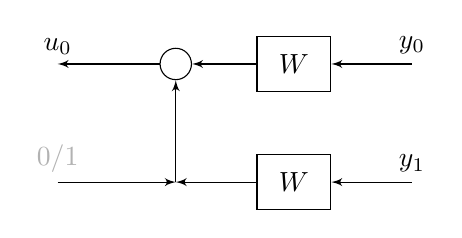
\begin{tikzpicture}[node distance = 1.5cm, auto]
      \coordinate (x0);
      \coordinate [below of=x0] (x1);
      \node [sum, right of=x0] (adder) {};
      \coordinate [below of=adder] (u1);
      \node [block, right of=adder] (chan0) {$W$};
      \node [block, right of=u1] (chan1) {$W$};
      \coordinate [right of=chan0] (y0);
      \coordinate [right of=chan1] (y1);
      
      \path [line] (adder) -- node [above, at end]{$u_0$}(x0);
      \path [line] (x1) -- node [above, at start, text opacity=.3]{$0 / 1$}(u1);
      \path [line] (u1) -- (adder);
      \path [line] (chan0) -- (adder);
      \path [line] (chan1) -- (u1);
      \path [line] (y0) -- node [above, at start]{$y_0$}(chan0);
      \path [line] (y1) -- node [above, at start]{$y_1$}(chan1);
    \end{tikzpicture}
  \caption{$W^2$ POLAR channel splitting}
  \label{fig:polar_split}
 \end{subfigure}%
\caption{POLAR channel construction}
\label{fig:polar_channel}
\end{figure}

\subsection{Channel construction}
First, channel combining is performed.
A POLAR encoder yields $W_N: \mathcal{X}^N \rightarrow \mathcal{Y}^N$ and the transition probalilities $W_N(y_1^N | x_1^N ) =  W^N (y_1^N |u_1^N G_N)$.
The second channel construction step is channel splitting.
It is depicted in Fig. \ref{fig:polar_split}.
For every $u_i$ of the vector channel, the conditional probalilities $W^{(i)}_N (y^N_1, u^{i-1}_1 | u_i)$ are calculated.
With this result the channel capacities $I (W^{(i)}_N )$ and Bhattacharyya parameters $Z ( W^{(i)}_N )$ are calculated.
The arrows in Fig. \ref{fig:polar_split} indicate the influence of $u^N_{i+1}$ and $y^N_1$ on the conditional probalilities of $u_i$.

\begin{figure}[htb]
  \centering
  \begin{subfigure}{.49\textwidth}
  \centering
   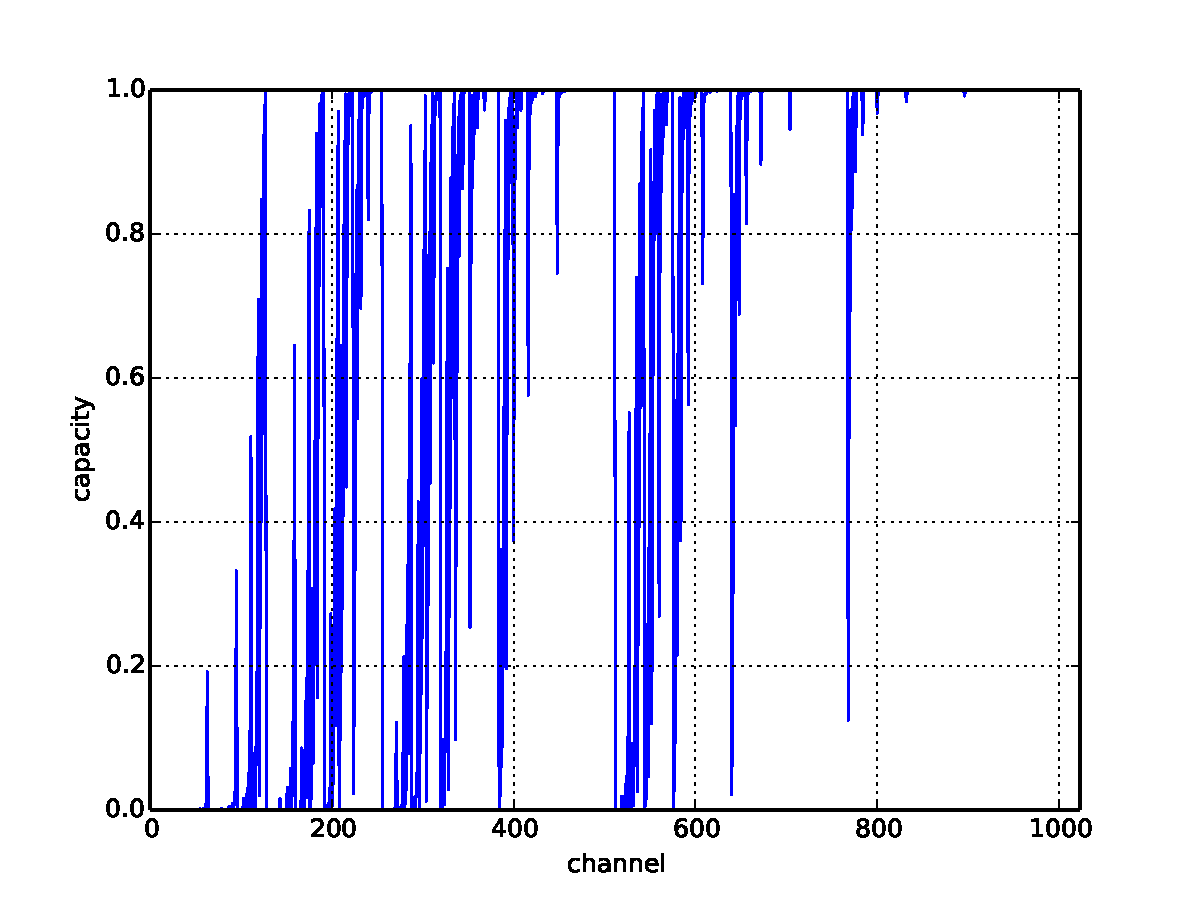
\includegraphics[width=\textwidth]{figure/bec_capacity_0_3_1024.pdf}
   \caption{\acs{BEC} $I (W^{(i)}_N )$ for $\eta=0.3$, $N=1024$}
   \label{fig:bec_capacity}
  \end{subfigure}
  \begin{subfigure}{.49\textwidth}
  \centering
   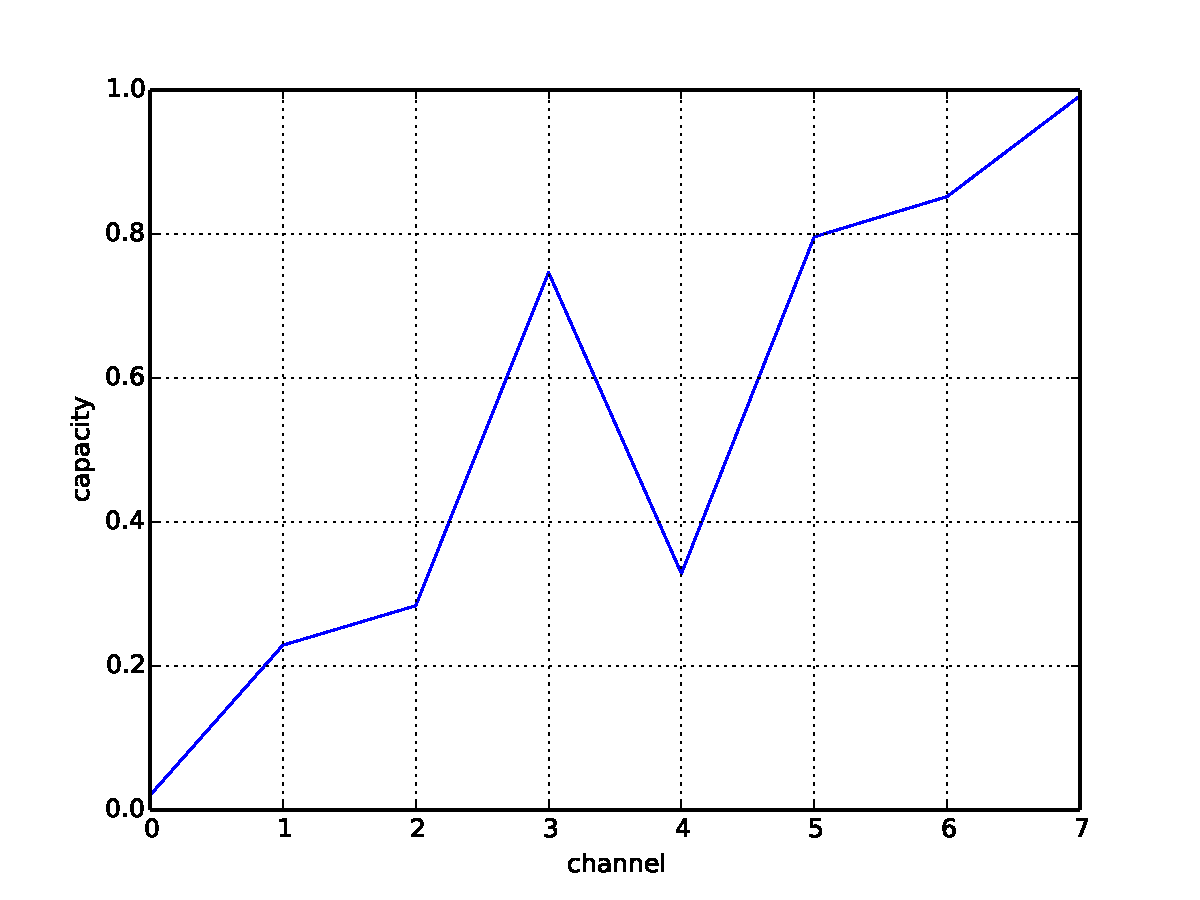
\includegraphics[width=\textwidth]{figure/bsc_capacity_0_1_8.pdf}
   \caption{\acs{BSC} $I (W^{(i)}_N )$ for $p=0.1$, $N=8$}
   \label{fig:bsc_capacity}
  \end{subfigure}
  \caption{Channel capacities for different channels}
  \label{fig:capacity}
\end{figure}

The polarization effect can be observed in Fig. \ref{fig:bec_capacity} and Fig. \ref{fig:bsc_capacity}.
The individual channels tend to $1.0$ or $0.0$ respectively.
Thus they are either perfect channels or noise-only channels.
A user chooses a desired rate and selects the best channels for \textit{information bits}.
All other channels will transmit \textit{frozen bits}.

Only \ac{BEC} channels can be calculated efficiently.
For other channels optimized algorithms are proposed in \cite{tal2013construct}.

\subsection{Decoder}
A successive interference cancellation (SIC) decoder is proposed to retrieve transmitted bits at the receiver.
This decoder operates at complexity $O( N log(N) )$.
It does not perform well for short block size, thus, a belief propagation (BP) decoder is also proposed by Arikan.
Several improved decoders are proposed in \cite{chen2013improved} and \cite{li2012adaptive} which further improve decoding performance.


% Describe which features will be implemented.
\section{Deliverables}
As an ESA Summer of Code in Space project I aim at contributing to GNU Radio a number of features.
I will outline those features in this section.

\paragraph{Integration} GNU Radio provides the gr-fec API to easily drop in channel codes.
FECAPI will be used to integrate POLAR codes directly into GNU Radio's gr-fec module.
Directly integrating POLAR codes should improve compatibility with other parts of the FECAPI.
This project will be available under the term of the GNU GPLv3.
At the end of the project a pull request for GNU Radio will be prepared in order to make POLAR codes available as easily as possible to every potential user.

\paragraph{Python test code} for extensive unit tests shall be created first.
This will foster my knowledge with POLAR codes and later serve as a reference in the unit test for the \CC{} implementation.

\paragraph{Encoders and Decoders} are the heart of the signal processing code.
They will be coded in \CC{} and seemlessly integrated into the FECAPI.
The integration of encoders and decoders is depicted in Fig. \ref{fig:polar_mockup}.
In order to make them as useful as possible they shall be optimized for maximum performance.

\begin{figure}[tbh]
 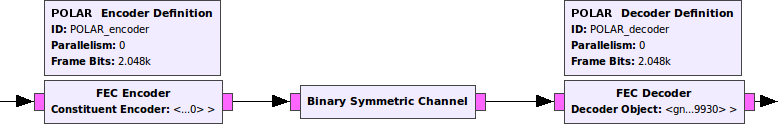
\includegraphics[width=\textwidth]{figure/POLAR_mockup.png}
 \caption{simple POLAR encoder/decoder flowgraph}
 \label{fig:polar_mockup}
\end{figure}

\paragraph{\acs{VOLK} kernels} will be created that use a \ac{CPU}'s \ac{SIMD} instruction set for further performance gains.
Those kernels will be prepared for merging with the \ac{VOLK} project.

\paragraph{Channel construction} for large codes will be implemented.
Therefore the proposed algorithms \cite{tal2013construct} will be implemented in Python using NumPy.
So users can parameterize there codes and then let the channel construction algorithms do the work to generate desired channel parameters.
In order to speed up usage, file save and file read will be provided.


\section{Timeline}
This is a preliminary timeline to give an overview of the upcoming project stages.
It is synchronized to the \ac{ESA} Summer of Code in Space timeline.

\paragraph{April 30} student application deadline.
\paragraph{May 1 - May 31 Community Bonding period} 4 weeks, gathering in-depth knowledge of the upcoming project, reading papers, documentation, meetings with mentor for detailed discussions.
Choose suitable algorithms for implementation.
\paragraph{June 1 - June 14 Initial Coding} 2 weeks, implement encoder, decoder and channel calculation for code construction in Python.
Create test suite for \CC{} implementation.
\paragraph{June 15 - June 29} 2 weeks, port encoder and decoder to gr-fec in GNU Radio.
Create blocks that can be dropped into the FECAPI framework and make all tests pass.
\paragraph{June 30 - July 5} 1 week, optimize encoder and decoder block for maximum throughput
\paragraph{July 6 - July 7 Mid-term wrap up} 2 days, prepare and submit results for mid-term evaluation.
\paragraph{July 8 - August 7} 4 weeks, implement \ac{VOLK} kernels for POLAR encoder and decoder.
\paragraph{August 8 - August 23} 2 weeks, implement sophisticated channel calculation algorithms to enable use of large vector channels.
\paragraph{August 24 pencils down} 1 week, issue pull request and work on integration into GNU Radio main.
\paragraph{August 31 project end} project hopefully merged in main.


\section{Motivation}
I am a Master degree student at \ac{KIT}, Germany.
My major is focused on Communication at \ac{CEL}.
Also I am currently a student research assistant at \ac{CEL}.
During my studies and work I acquired advanced skills in digital signal processing, waveform design and software engineering.

I got in touch with GNU Radio back in 2012 when I started my Bachelor thesis on {\ac{LTE} signal reception with GNU Radio}.
The outcome of this thesis is available on Github \cite{repo:gr-lte}.
After I finished my Bachelor thesis I continued to work on it and added more features as well as code improvements.
Further outcome of this work are two articles \cite{lte:winncomm2013} and \cite{lte:springer2015}.
During the course of gr-lte development I touched a great variety of different parts of GNU Radio.
Firstly adopting and integrating existing blocks into the project.
Secondly learning a lot about GNU Radio internals like scheduler specifics, class inheritance structures and \ac{VOLK} usage.
Also, I improved my knowledge to write test code in order to improve code quality.

Besides my studies at \ac{KIT} I did an internship at Ettus Research in 2013/14, fostering my programming skills and deepening my GNU Radio knowledge.
During that time I contributed to Ettus' UHD driver and developed tools for use with GNU Radio \cite{repo:gr-misc}.

Currently I'm working as a student research assistant at \ac{CEL} again.
My fields of interest are \ac{SDR} development and system optimization.
This includes heavy algorithmic optimization and overall code optimization for maximum throughput and bandwidth capabilities.
Recently I contributed to GNU Radio by adding a rename capability to its modtool tool \cite{repo:gr-rename-contribution}.

Besides my experience with GNU Radio and thus with \CC{} and Python, I also did several smaller projects.
That includes closed source projects at university level with Java and Java for Android.
I did microcontroller programming in ANSI C and Assembler.
This included integration of an IP microcontroller into an existing VHDL project.

Before \ac{ESA} Summer of Code in Space starts I will have finished my last exams and be fully available for my project.
I want to take the opportunity to work on GNU Radio while I am still a student.
Also, I aim at using the results of my project as part of my Master thesis.
I hope to foster my knowledge and experience with software engineering and channel coding.

During the course of the project, I will have access to \ac{CEL}'s labs and equipment.
And Sebastian Koslowski, who is currently with \ac{CEL}, agreed on mentoring my project.
Thus I will always be able to talk to him personally about project progress and pitfalls.

I read GNU Radio's Code of Conduct and understood and agree to it, including the three strikes rule.
They are natural to follow and essential for a positive and prospering community.
I am looking forward to publish my weekly project updates.

GNU Radio is an amazing tool to rapidly develop new waveforms.
I would be more than happy to contribute to it so others can benefit from my work, just as I do from having GNU Radio at hand.
Furthermore, I want to use the opportunity to enable development of new channel codes in the hope that one day, they will go to space.

\section{Conclusion}
Channel codes are a crucial component of every communication system.
High performance codes enable reliable high bandwidth data transmission.
It is often very difficult to choose an appropriate channel code for a specific use-case.
Therefore it is beneficial to have a variety of different implementations at hand, especially for GNU Radio with a strong focus an research and development.
Having POLAR codes as an option for channel codes in GNU Radio enables users to evaluate this code for use in many different environments, such as in space.
A fast POLAR code implementation for GNU Radio will ease user's lives to conduct tests.
POLAR codes are an exciting field for further investigations because they promise to reach Shannon channel capacity.

I would like to take this opportunity to participate in GNU Radio development and contribute to it.


\newpage
\appendix
  \bibliography{litverz}	% Literaturverzeichnis (litverz.bib)

  % Am besten einen dieser bibliographystyle's auswaehlen
%  \bibliographystyle{geralpha}
%  \bibliographystyle{alpha}
%  \bibliographystyle{unsrt}
\bibliographystyle{IEEEtran}

% For use with acronym package
% \acrodef{⟨acronym⟩}[⟨short name⟩]{⟨full name⟩}

\section{Abbreviations}
\begin{acronym}[TROLL]
 \acro{ESA}[ESA]{European Space Agency}
 \acro{NASA}[NASA]{National Aeronautics and Space Administration}
 \acro{LDPC}[LDPC]{Low-Density Parity-Check}
 \acro{SIMD}[SIMD]{Single Instruction Multiple Data}
 \acro{VOLK}[VOLK]{Vector-Optimized Library of Kernels}
 \acro{BDMC}[BDMC]{symmetric binary discrete memoryless channel}
 \acro{BSC}[BSC]{Binary Symmetric Channel}
 \acro{BEC}[BEC]{Binary Erasure Channel}
 \acro{CPU}[CPU]{Central Processing Unit}
 \acro{KIT}[KIT]{Karlsruhe Institute of Technology}
 \acro{CEL}[CEL]{Communications Engineering Lab}
 \acro{LTE}[LTE]{Long Term Evolution}
 \acro{SDR}[SDR]{Software-Defined Radio}
\end{acronym}


\end{document}
